\documentclass[12pt]{article}

% --- Geometry & Fonts ---
\usepackage[letterpaper, margin=0.5in]{geometry}
\usepackage[T1]{fontenc}
\usepackage{helvet}
\renewcommand{\familydefault}{\sfdefault}

% --- Packages ---
\usepackage[utf8]{inputenc}
\usepackage{booktabs}
\usepackage{graphicx}
\usepackage{amsmath}
\usepackage{hyperref}
\usepackage{xcolor}
\usepackage{tabularx}
\usepackage{float}
\usepackage{enumitem}
\usepackage{caption}

\graphicspath{{../images/}}

\hypersetup{
    colorlinks=true,
    linkcolor=blue!70!black,
    urlcolor=blue!70!black,
    citecolor=blue!70!black
}

% --- Compact spacing ---
\usepackage{titlesec}
\titlespacing*{\section}{0pt}{8pt}{4pt}
\setlength{\parskip}{3pt}
\setlength{\parindent}{0pt}
\setlength{\abovecaptionskip}{4pt}
\setlength{\belowcaptionskip}{2pt}
\setlength{\textfloatsep}{6pt}
\setlength{\floatsep}{6pt}
\setlength{\intextsep}{6pt}
\setlist{nosep, leftmargin=1.5em}

% --- Title ---
\title{\vspace{-2cm}\textbf{Prototype Verification Summary --- Team 0109D}\vspace{-0.5cm}}
\author{ESC204 Design Dossier \textnormal{--- Artifact 04.4}}
\date{\vspace{-0.5cm}}

\begin{document}
\maketitle
\thispagestyle{empty}

%=============================================================================
\section{Verification Overview}
%=============================================================================

All prototype subsystems were validated through a structured, three-test empirical protocol followed by a mechanical endurance stress test. The sequence was deliberately ordered by increasing realism and difficulty: \textbf{Test~1} (Output Force Quantification) established baseline force magnitudes across nozzle geometries; \textbf{Test~2} (Distance \& Angle Optimization) characterized clearing performance on a high-friction roof mock-up at varying standoff distances; and \textbf{Test~3} (Wet Debris Maximum Stiction) subjected the system to worst-case saturated debris conditions. A final \textbf{Endurance Test} verified that the integrated stepper-driven track could sustain continuous automated operation without mechanical or thermal failure.

%=============================================================================
\section{Test 1 --- Output Force Quantification}
%=============================================================================

\textbf{Setup.} A Dyson hairdryer at maximum airflow setting directed its output onto a $14 \times 14$\,cm rigid target resting on a digital scale. Four nozzle geometries were tested at standoff distances of 4\,cm, 8\,cm, 12\,cm, and 16\,cm.

\begin{table}[H]
\centering
\caption{Measured output force (N) by nozzle geometry and standoff distance.}
\label{tab:test1}
\begin{tabular}{@{}lcccc@{}}
\toprule
\textbf{Nozzle Geometry} & \textbf{4\,cm} & \textbf{8\,cm} & \textbf{12\,cm} & \textbf{16\,cm} \\
\midrule
Pure Dyson (Baseline)    & 1.96 & 1.95 & 1.95 & 1.76 \\
Dyson OEM Air Blade      & 1.98 & 1.97 & 1.95 & 1.78 \\
Custom Air Blade          & 1.96 & 1.95 & 1.93 & 1.72 \\
Double-Sided Air Blade    & 1.91 & 1.88 & 1.85 & 1.62 \\
\bottomrule
\end{tabular}
\end{table}

\textbf{Key Finding.} Total aerodynamic force is conserved at approximately 1.96\,N ($\approx$200\,g) across all single-exit geometries within 12\,cm. Nozzle geometry \emph{redistributes} the momentum flux into a planar shear layer but does not increase it. The sharp degradation observed at 16\,cm establishes a hard operational constraint: the nozzle must remain within 12\,cm of the target surface.

%=============================================================================
\section{Test 2 --- Distance \& Angle Optimization}
%=============================================================================

\textbf{Setup.} A $35 \times 15$\,cm roof mock-up covered in 40-grit aluminum oxide sandpaper (simulating asphalt shingle friction) was locked at a $30^\circ$ incline. A custom alignment frame with protractor ensured nozzle parallelism to the roof pitch; axial alignment was independently verified by a second observer. Disaggregated dry tissue paper served as the debris analogue. Three trials were conducted per configuration at $d = 10$\,cm, 25\,cm, and 50\,cm.

\begin{table}[H]
\centering
\caption{Clearing performance: Circular Nozzle vs.\ Custom Air Blade at $30^\circ$.}
\label{tab:test2}
\begin{tabularx}{\textwidth}{@{}lXX@{}}
\toprule
\textbf{Distance} & \textbf{Circular Nozzle} & \textbf{Custom Air Blade} \\
\midrule
$d = 10$\,cm &
Full clearance; instantaneous impact force sufficient regardless of geometry. &
Full clearance; geometry advantage negligible at close range. \\
\addlinespace
$d = 25$\,cm &
Partial clearance; central debris ejected but lateral residue remains. &
Superior ejection height and distance; planar shear layer penetrates \emph{under} debris. \\
\addlinespace
$d = 50$\,cm &
Narrow central path cleared only; severe turbulent diffusion leaves lateral residue across the 15\,cm width. &
Wide, uniform sweep clears full 15\,cm width; coherent planar jet resists diffusion. \\
\bottomrule
\end{tabularx}
\end{table}

\textbf{$\boldsymbol{30^\circ}$ Angle Justification.} At $30^\circ$, the airflow vector decomposes into a normal component $F_y$ (sufficient for Coanda boundary-layer attachment without pinning the debris) and a maximized tangential shear component $F_x$ (driving debris down the slope). Angles exceeding $45^\circ$ amplify $F_y$ to the point of pinning; angles below $15^\circ$ cause the stream to deflect over the debris profile without engagement.

%=============================================================================
\section{Test 3 --- Wet Debris Maximum Stiction}
%=============================================================================

\textbf{Setup.} Identical to Test~2 at $d = 50$\,cm, but with \emph{heavily saturated} tissue paper to maximize static friction and minimize the aerodynamic profile available for dislodgement.

\begin{itemize}
    \item \textbf{Circular Nozzle --- FAILED.} The localized high-pressure column pinned wet tissues flat against the 40-grit surface. Only marginal central dislodgement was observed.\\
    Video: \href{https://drive.google.com/file/d/1wO-Wh8iFGygEvBvc3OOH91XQSwhoY_Ws/view}{Circular Nozzle Wet Trial}
    \item \textbf{Custom Air Blade --- PASSED.} The high-velocity planar shear layer slipped beneath the water/sandpaper barrier and peeled saturated debris off the surface.\\
    Video: \href{https://drive.google.com/file/d/16htpF3ptwKEM5UxYE679x3f3xWmt80h1/view}{Air Blade Wet Trial}
\end{itemize}

\textbf{Full trial set (8 videos):} \href{https://drive.google.com/drive/folders/1RAJA95EF-XjMrkhjWkuoIBbONH_DbRVu}{View Google Drive Folder}

\begin{figure}[H]
\centering
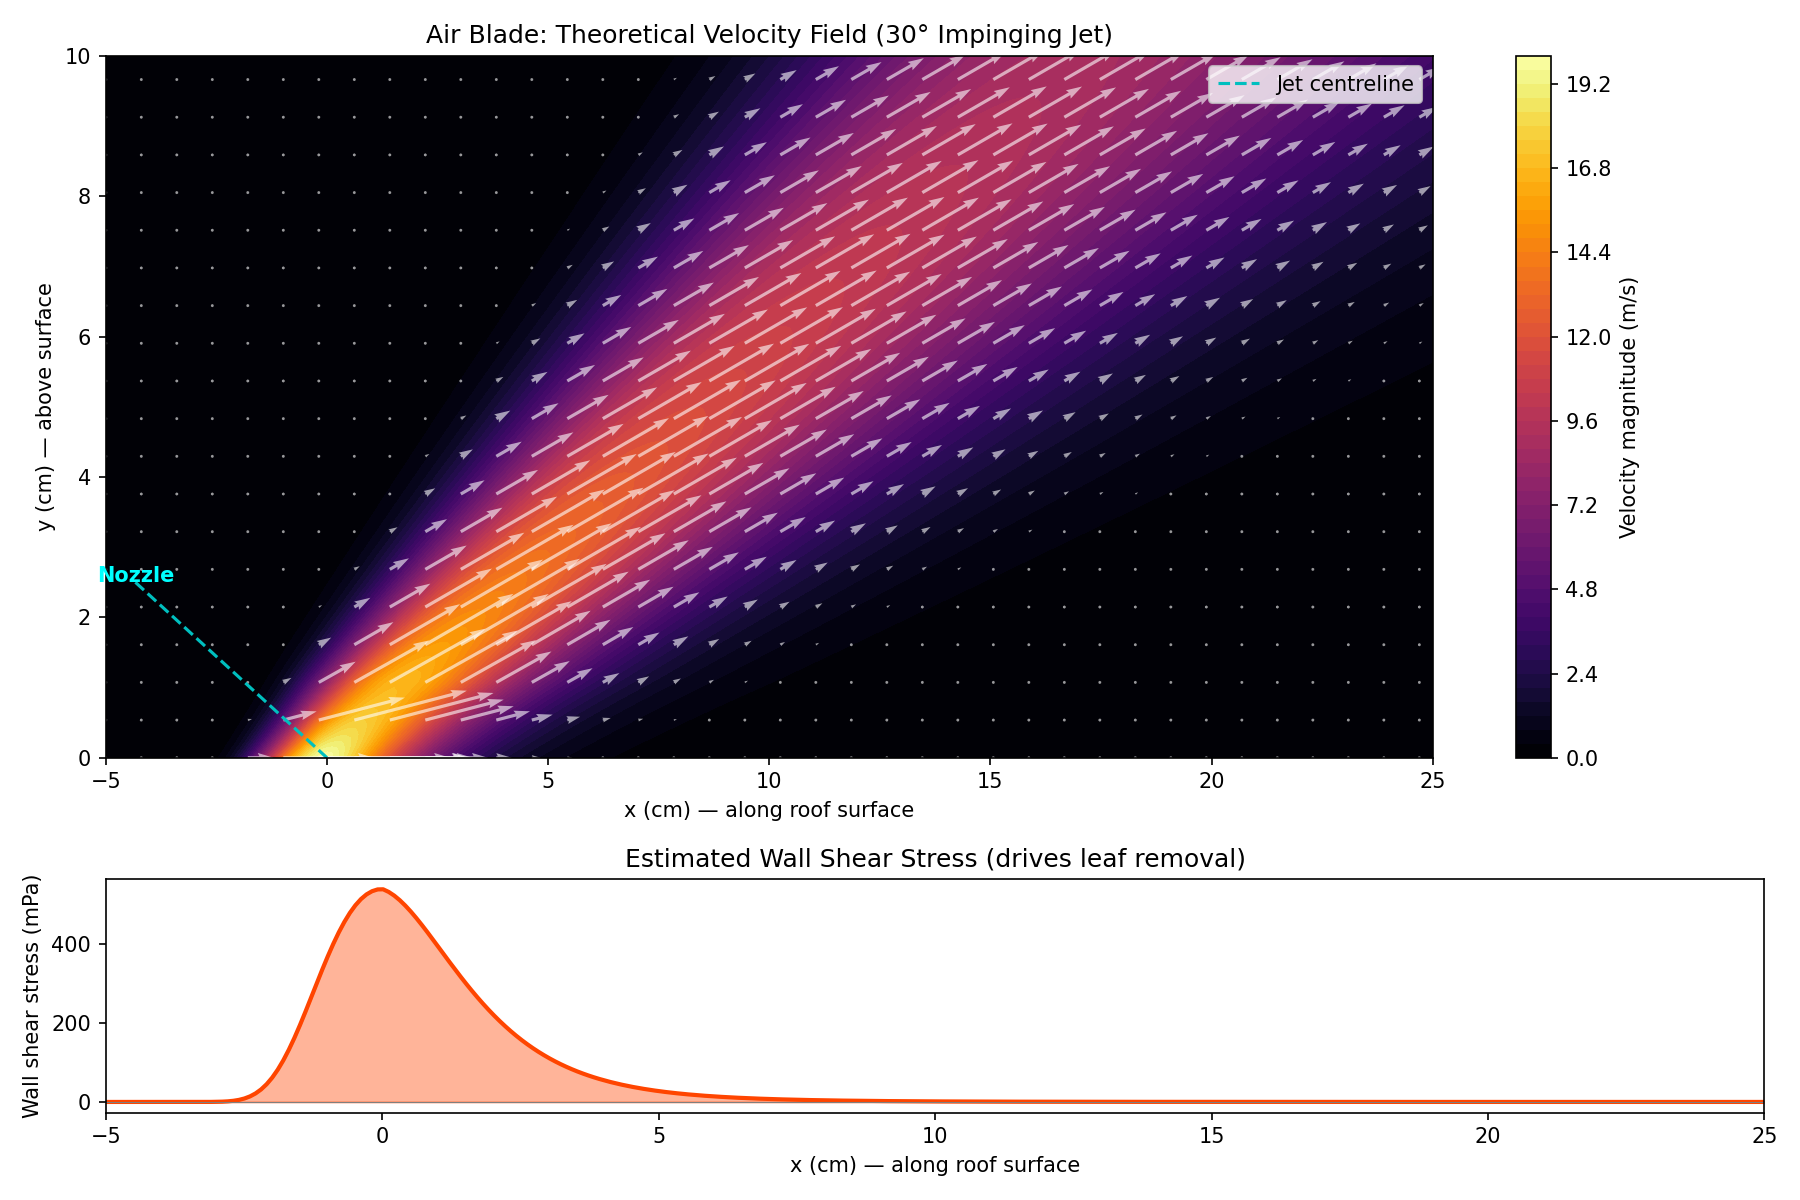
\includegraphics[width=0.55\textwidth]{shear_layer_visualization.png}
\caption{Shear-layer visualization illustrating the planar jet's ability to penetrate under low-profile debris.}
\label{fig:shear}
\end{figure}

%=============================================================================
\section{Endurance Testing}
%=============================================================================

The fully integrated stepper-driven track was subjected to a continuous 2-minute operational cycle, exceeding the minimum 2-pass verification threshold. Results:

\begin{itemize}
    \item \textbf{Stalling:} Zero instances across 120\,s of continuous operation.
    \item \textbf{Belt tension:} Maintained through all direction reversals triggered by limit switches.
    \item \textbf{Thermal:} A4988 stepper driver remained within safe operating limits ($V_{\text{REF}}$ tuned to $\sim$50\% capacity).
    \item \textbf{Measured traverse:} 56\,cm in 22\,s $\;\Rightarrow\; v \approx 2.55$\,cm/s linear carriage velocity.
\end{itemize}

\textbf{Video:} \href{https://drive.google.com/drive/folders/1wNK_jYUvHXoMne_cIdYbAIURdvYpuG-J}{Endurance Test Folder}

%=============================================================================
\section{Specification Compliance}
%=============================================================================

All eleven design specifications were verified and passed. Table~\ref{tab:specs} summarizes the compliance status.

\begin{table}[H]
\centering
\caption{Specification compliance matrix --- all requirements satisfied.}
\label{tab:specs}
\begin{tabular}{@{}llc@{}}
\toprule
\textbf{Spec ID} & \textbf{Domain} & \textbf{Status} \\
\midrule
O-1.1-ELEC-1 & Electrical & \textcolor{green!50!black}{\textbf{PASS}} \\
O-2.1-ELEC-1 & Electrical & \textcolor{green!50!black}{\textbf{PASS}} \\
O-2.2-ELEC-1 & Electrical & \textcolor{green!50!black}{\textbf{PASS}} \\
O-3.2-ELEC-1 & Electrical & \textcolor{green!50!black}{\textbf{PASS}} \\
\addlinespace
O-1.1-STRU-1 & Structural & \textcolor{green!50!black}{\textbf{PASS}} \\
O-1.1-STRU-2 & Structural & \textcolor{green!50!black}{\textbf{PASS}} \\
O-4.1-STRU-1 & Structural & \textcolor{green!50!black}{\textbf{PASS}} \\
O-4.2-STRU-1 & Structural & \textcolor{green!50!black}{\textbf{PASS}} \\
\addlinespace
O-1.3-SOFT-1 & Software   & \textcolor{green!50!black}{\textbf{PASS}} \\
O-2.1-SOFT-1 & Software   & \textcolor{green!50!black}{\textbf{PASS}} \\
O-3.2-SOFT-1 & Software   & \textcolor{green!50!black}{\textbf{PASS}} \\
\bottomrule
\end{tabular}
\end{table}

\vfill
\begin{center}
\small\textit{All supporting video evidence is archived on the team Google Drive and linked inline above.}
\end{center}

\end{document}
